\documentclass[11pt,twocolumn,letterpaper,spanish]{article}
\usepackage[utf8]{inputenc}
%\usepackage{mathptmx} %Fuente Times New Roman
\usepackage[spanish,mexico]{babel}
\usepackage[left=2.5cm,right=2.5cm,top=2.5cm,bottom=2.5cm]{geometry}
\usepackage{lipsum}

%Para tabular
\usepackage{mwe} %Para que la imagen en la tabla se centre
\usepackage{graphbox} %Para que la imagen en la tabla se centre
\usepackage{array} %Para que se pueda centrar el texto en la tabla
\usepackage{booktabs}%Formato de celdas de Excel
\usepackage{multirow}%Formato de multiples filas de Excel


%Paquetes de la American Mathematical Society
\usepackage{amsmath,amsfonts,amssymb}

%insertar imagenes
\usepackage{graphicx}

%insertar imagenes en dos columnas
\usepackage{stfloats}

%Texto rodea figuras
\usepackage{wrapfig}

%Parrafos sin indentación
\setlength\parindent{0pt}


%Pone el título del abstract de buen tamaño
\makeatletter
\renewenvironment{abstract}{%
    \if@twocolumn
      \section*{\abstractname}%
    \else %% <- here I've removed \small
      \begin{center}%
        {\bfseries \Large\abstractname\vspace{\z@}}%  %% <- here I've added \Large
      \end{center}%
      \quotation
    \fi}
    {\if@twocolumn\else\endquotation\fi}
\makeatother


%Citar en APA
\usepackage{apacite}

\begin{document}

\begin{titlepage}

  
\includegraphics[width=2.8cm]{Logos/uady.jpg}
  \hfill
  
\includegraphics[width=4.4cm]{Logos/filogo.png}
  
  \hfill
   
    \begin{center}       
 
        \Huge
        \textbf{Reporte de práctica}
         
        \vspace{0.25cm}
        
        \LARGE
        Datalogger de temperatura
        \vspace{2.5cm}
        
        
		\LARGE \textbf{Universidad Autónoma de Yucatán\\}
        Facultad de Ingeniería\\        
        
        \vspace{1.5cm}
 
        \textbf{Saúl Eliseo Gamboa León}\\
        \vspace{0.2cm}
        Estudiante de Ingeniería Física
        
        \vspace{1.5cm}
        
        \textbf{Prof. Enrique Camacho Pérez}\\
        \vspace{0.2cm}
        Adquisición de datos
 
        \vspace{2cm}
 
        
 
        \LARGE
        Mérida, Yucatán\\
        26 de Junio de 2019
     
        
    \end{center}
\end{titlepage}

\twocolumn[
  \begin{@twocolumnfalse}
  \begin{abstract}
  {\large 
  
  	\noindent Se armó un datalogger de bajo costo utilizando módulos de reloj y memoria Micro-SD, una placa Arduino y sensores de temperatura. En equipos se realizó el armado de estos sistemas y se realizó la medición de temperatura de una lata de aluminio por cada equipo. Las latas utilizadas eran de distintos colores, con esto se buscó comparar la absorción de radiación de cada color durante el post-análisis. El guardado de información de tiempo y temperatura fue favorable. Durante el análisis de utilizaron librerias del lenguaje Python para graficar los valores medidos de temperatura contra la hora-minuto del día en el que fue tomado cada valor; la gráfica se comportó como se esperaba, con picos de temperatura durante las horas más activas del sol y disminuyendo considerablemente en la noche. La lata que mayor temperatura mostró en dichas gráficas fue la pintada de negro, lo cual de nuevo nos indica que las mediciones fueron correctas.
  }\end{abstract}
  \end{@twocolumnfalse}
]

\section*{Introducción}

\vspace{-1.55 cm}

Un registrador de datos (también llamado data logger de datos o recopilador de datos) es un dispositivo electrónico que registra datos a lo largo del tiempo o en relación con la ubicación, ya sea con un instrumento o sensor incorporado o mediante instrumentos y sensores externos. Cada vez más, pero no del todo, se basan en un procesador digital (o computadora). Por lo general, son pequeños, funcionan con batería, son portátiles y están equipados con un microprocesador, memoria interna para almacenamiento de datos y sensores. Algunos registradores de datos pueden interaccionar con una computadora personal y utilizan un software para activar el registrador de datos, ver y analizar los datos recopilados, mientras que otros tienen un dispositivo de interfaz local (teclado, LCD) y se pueden usar como dispositivos independientes \cite{goyaldata}

Los registradores de datos se basan en un procesador digital. Es un dispositivo electrónico que registra datos a lo largo del tiempo en relación con la ubicación, ya sea con un instrumento o sensor incorporado, o mediante instrumentos y sensores externos. El data logger puede recopilar datos automáticamente las 24 horas, este es el principal y el más Importante beneficio de usar los registradores de datos \cite{Badhiye}


\section*{Objetivo}

Construir un datalogger que registre la información de temperatura del agua dentro de una lata de aluminio colocada a la intemperie durante un periodo aproximado de 24 horas.

\section*{Hipótesis}

\begin{itemize}
\item La temperatura registrada será mayor para las horas en las cuales el sol se encuentre en su cenit y disminuirá conforme diverja de dicha posición.
\item Las latas pintadas con colores más oscuros absorberán mayor cantidad de radiación
\end{itemize}

\section*{Materiales}

En la Tabla 1 se muestran imágenes y el nombre de los materiales utilizados para la construcción del datalogger

\begin{table*}[hbt!]
  \centering
  \begin{tabular}{ m{6cm}  m{3.5cm} }
    \toprule
    Material  & Imagen \\
    \midrule
      Arduino Nano y cable USB & 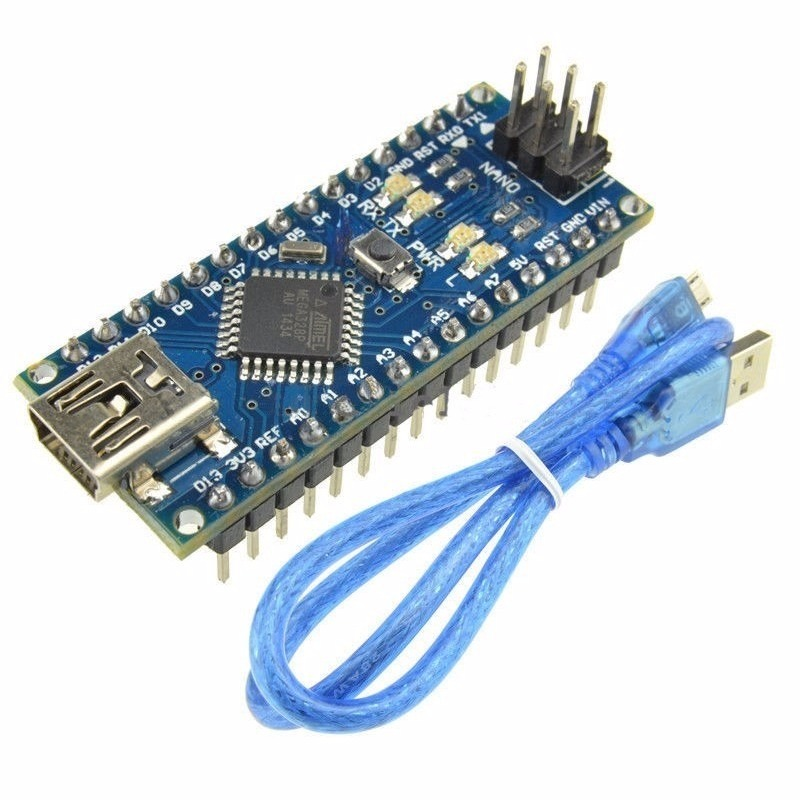
\includegraphics[align=t,scale=0.09]{Materiales/nano}\\
      \hline
      Módulo de memoria SD & 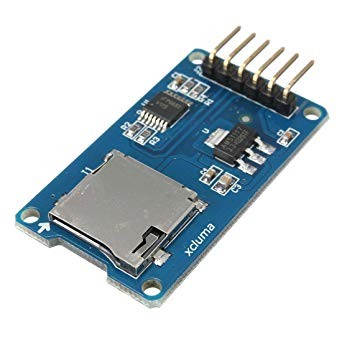
\includegraphics[align=t,scale=0.16]{Materiales/sd}\\
      \hline
      Módulo de reloj a tiempo real D1302 & 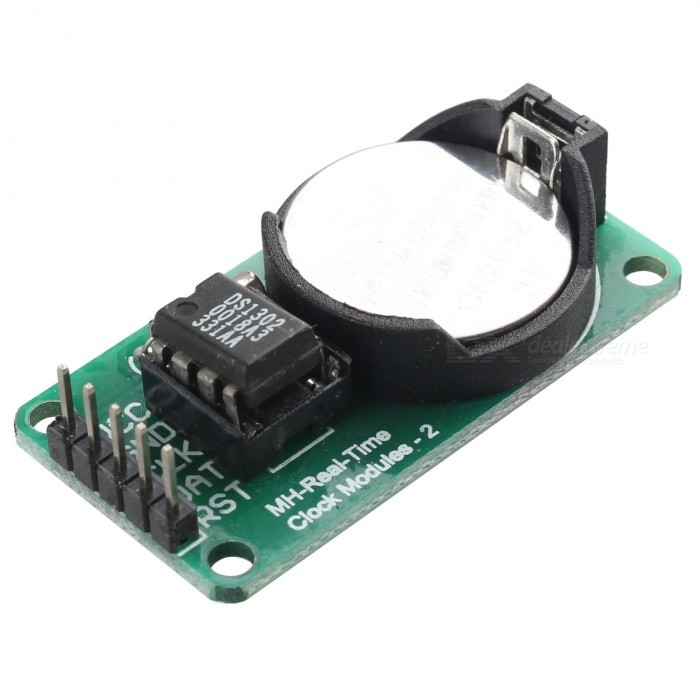
\includegraphics[align=t,scale=0.09]{Materiales/reloj}\\
      \hline
      Sensor de temperatura DS18B20 & 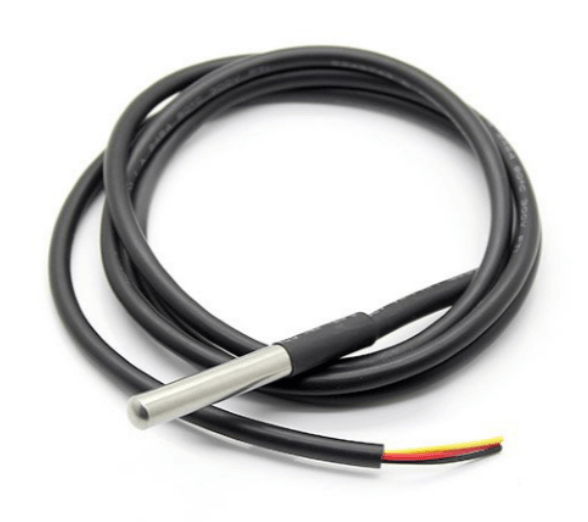
\includegraphics[align=t,scale=0.1]{Materiales/tempsen}\\
      \hline
      Protoboard & 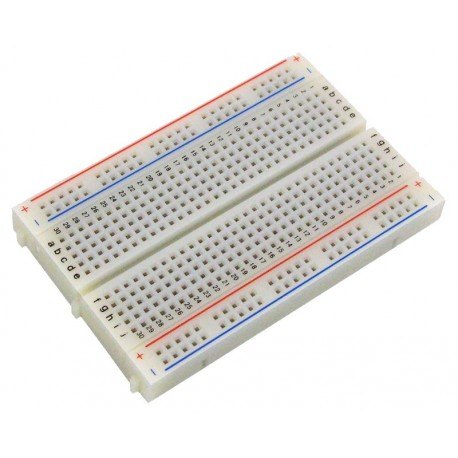
\includegraphics[align=t,scale=0.15]{Materiales/proto}\\
      \hline
      Cables dupont & 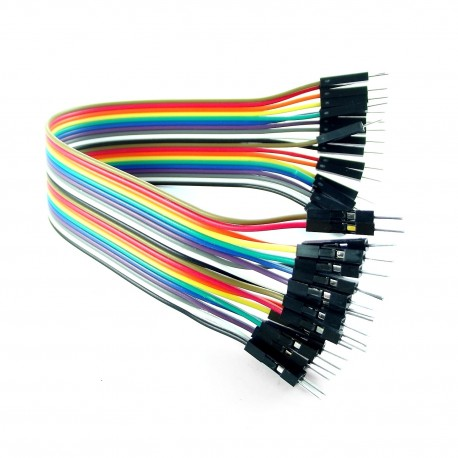
\includegraphics[align=t,scale=0.14]{Materiales/dupont}\\
      \hline
      Lata de aluminio & 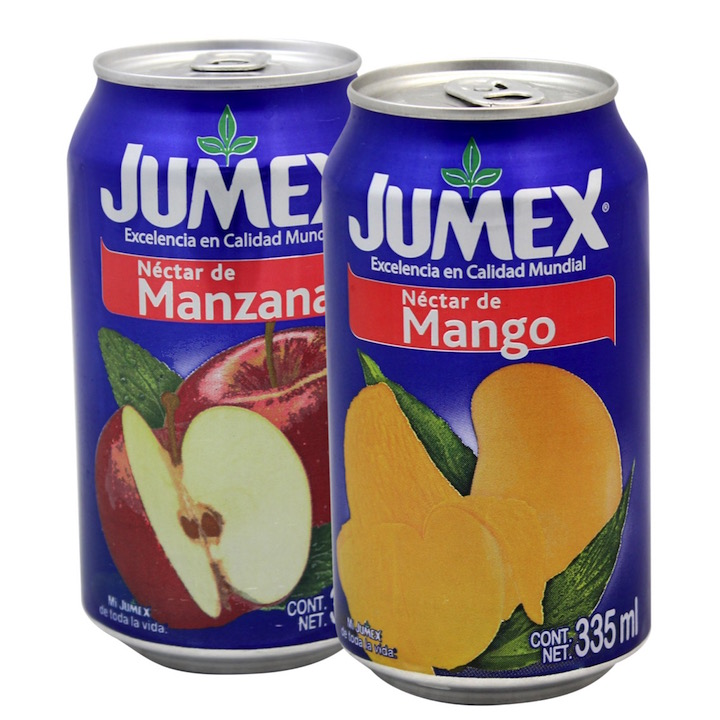
\includegraphics[align=t,scale=0.08]{Materiales/lata}\\
      \hline
      Caja de plástico & 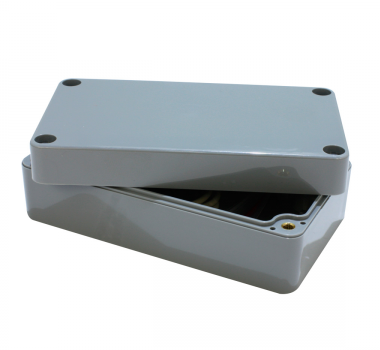
\includegraphics[align=t,scale=0.16]{Materiales/cajita1}\\
      \hline
      Adaptado de corriente para celular & 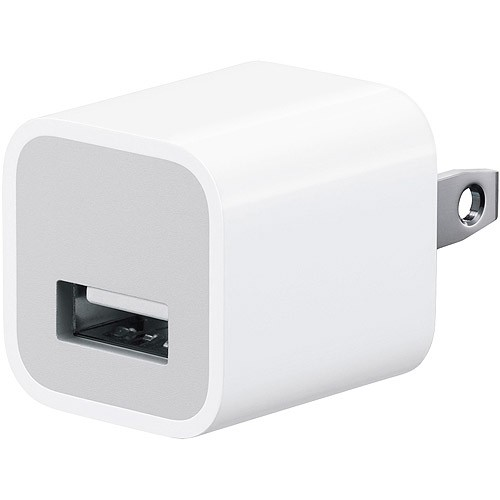
\includegraphics[align=t,scale=0.10]{Materiales/adaptador}\\
    \bottomrule
  \end{tabular}
  \caption{Materiales utilizados para el data logger}
\end{table*}


\section*{Metodología}

\begin{enumerate}
\item Se realizaron la conexiones pertinentes sobre una protoboard del Arduino nano al sensor DS18B20, el módulo de lectura de memoria microSD y el reloj DS1302. En la Figura 1 se muestra la esquemática del circuito.

\begin{figure}[h!]
   \centering
   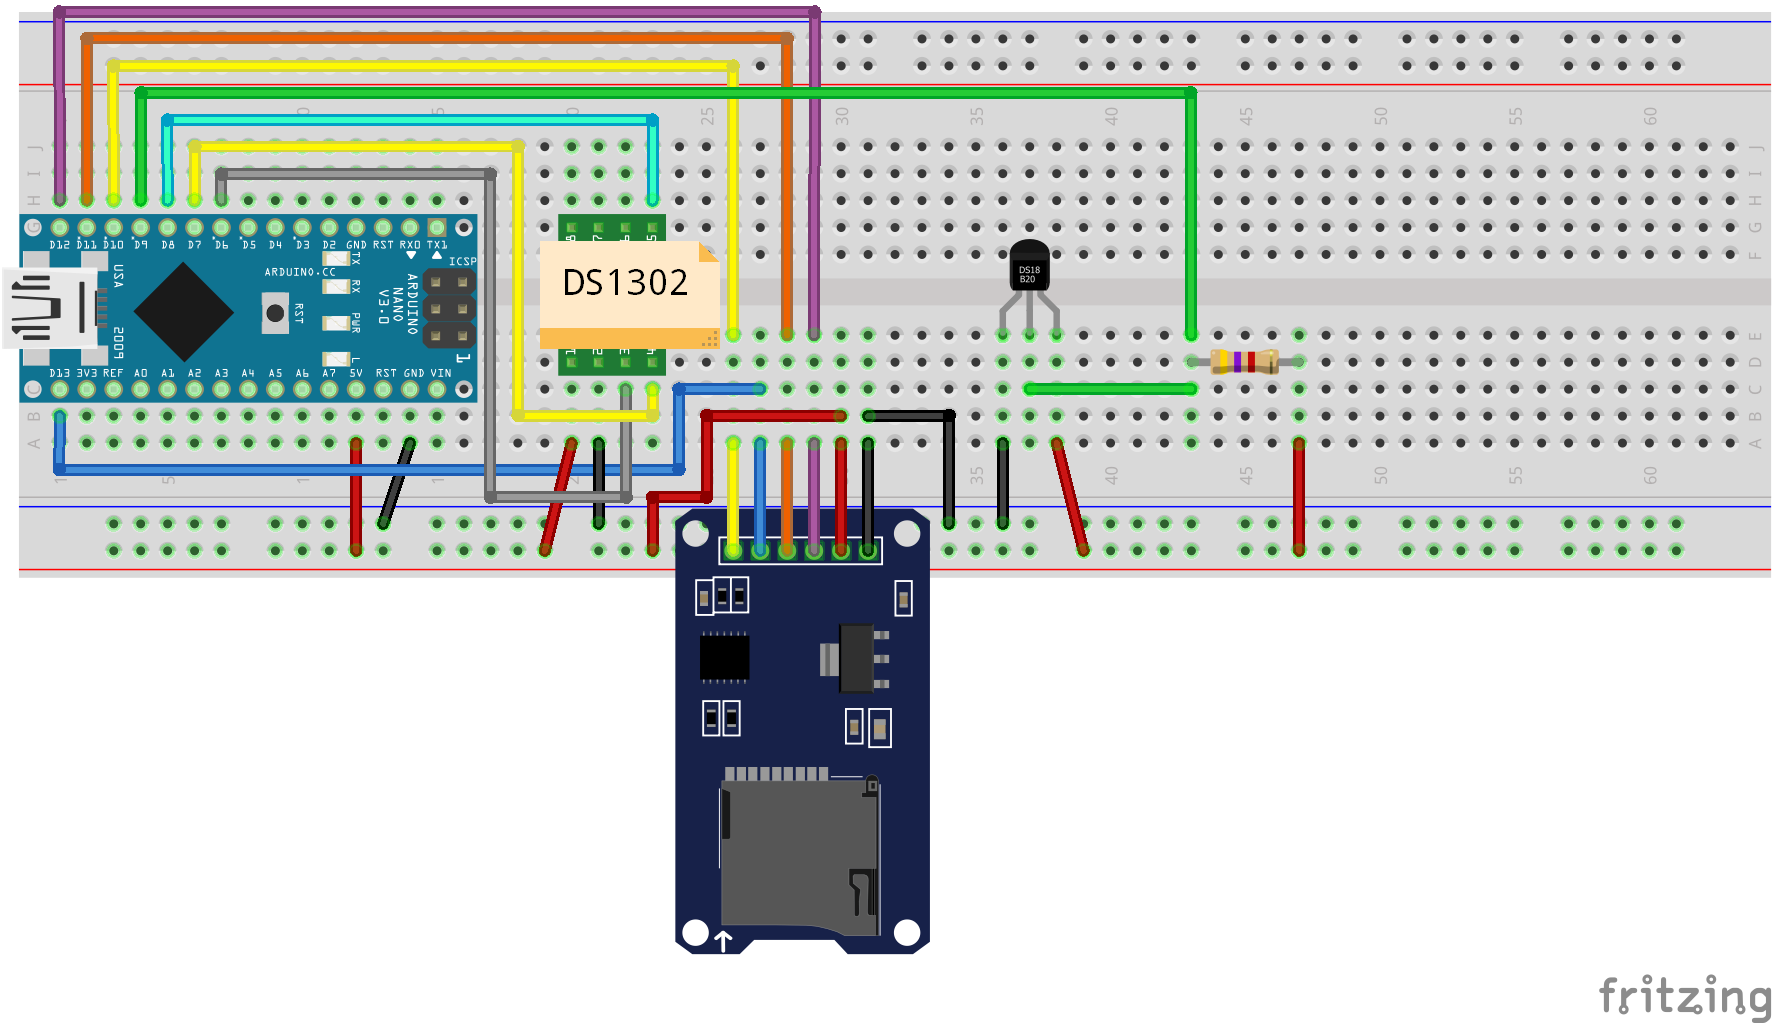
\includegraphics[width = 6.5 cm,height = 4 cm]{Imagenes/esquema}
   \caption{Esquemática del data logger}
\end{figure}


\item Se cargó en el Arduino Nano el código necesario para recopilar la fecha, hora y temperatura a cada segundo dentro de un archivo de texto en la memoria microSD del data logger.

\begin{figure}[h!]
   \centering
   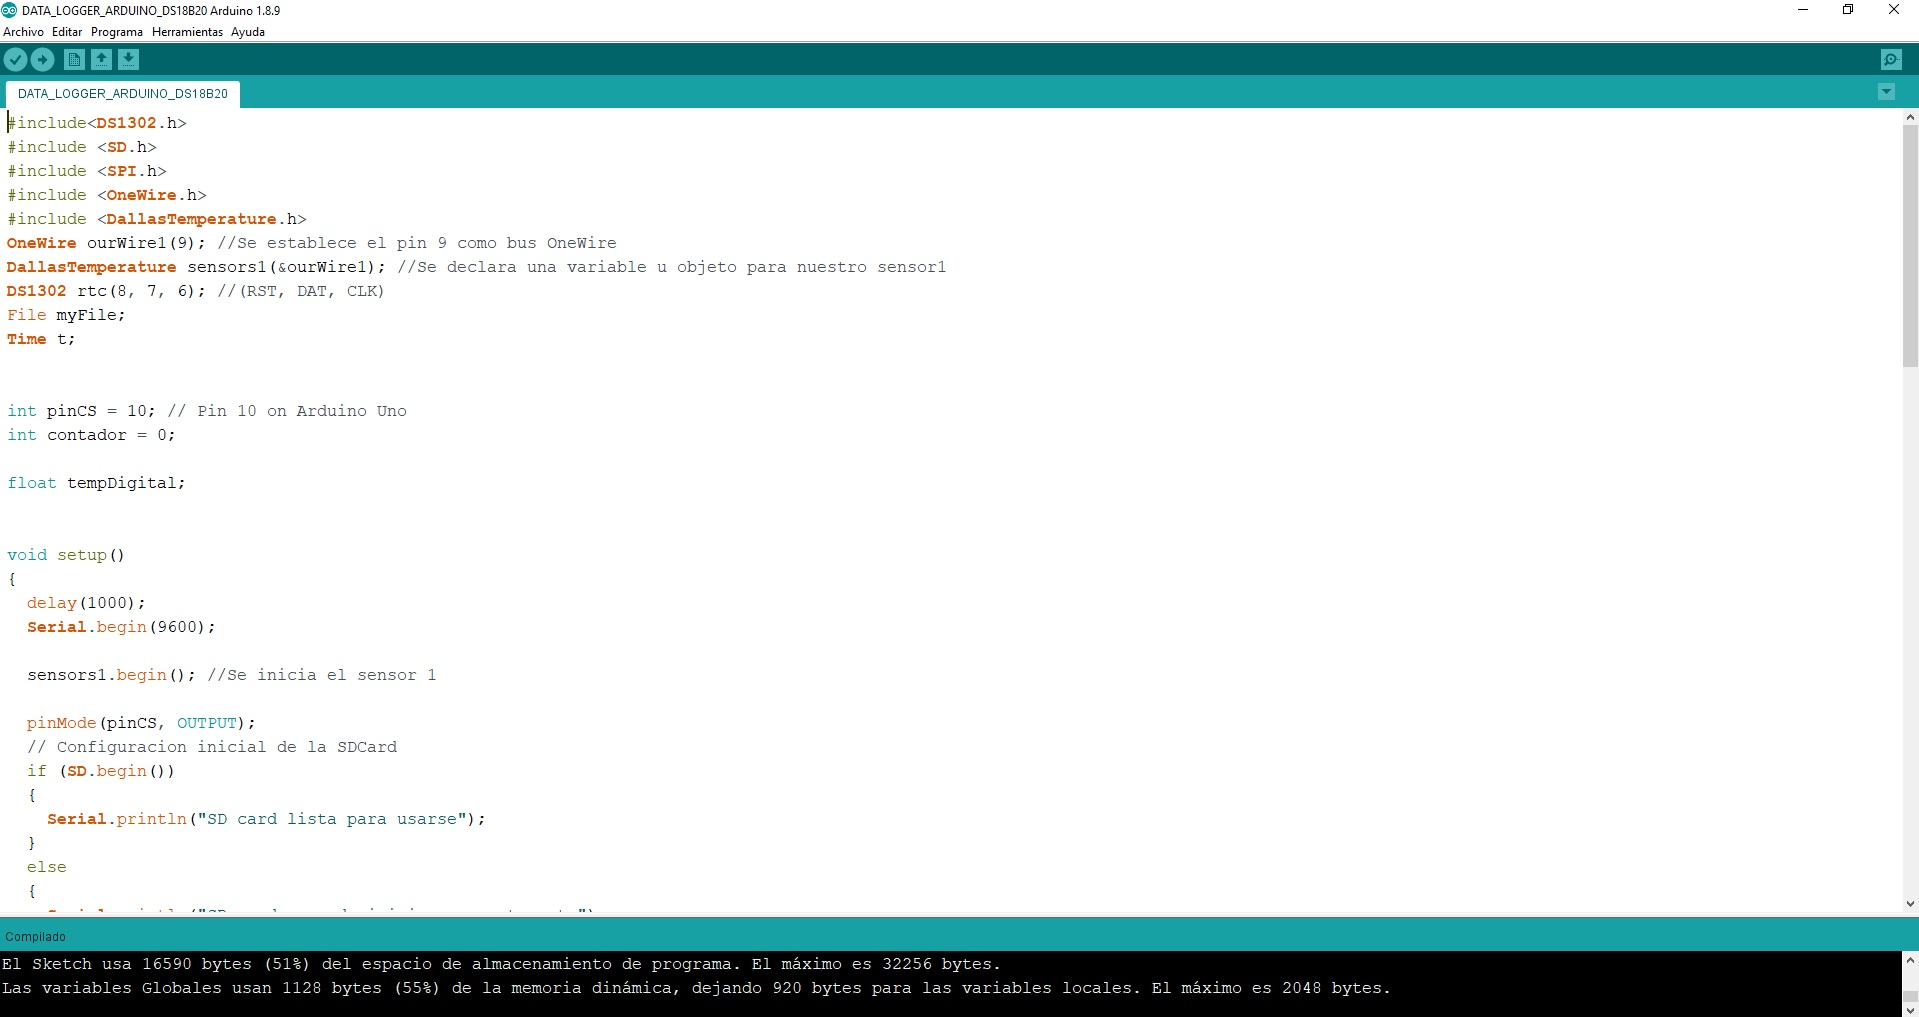
\includegraphics[width = 7 cm, height = 5 cm]{Imagenes/arduinoide}
   \caption{IDE Arduino con el código del data logger}
\end{figure}

\item En el caso del equipo 7, se colocó el data logger dentro de una pequeña caja de plástico con apertura en el lado izquierdo para que pudieran salir el sensor de temperatura y el cable de alimentación para el Arduino como se muestra en la figura 3

\begin{figure}[h!]
   \centering
   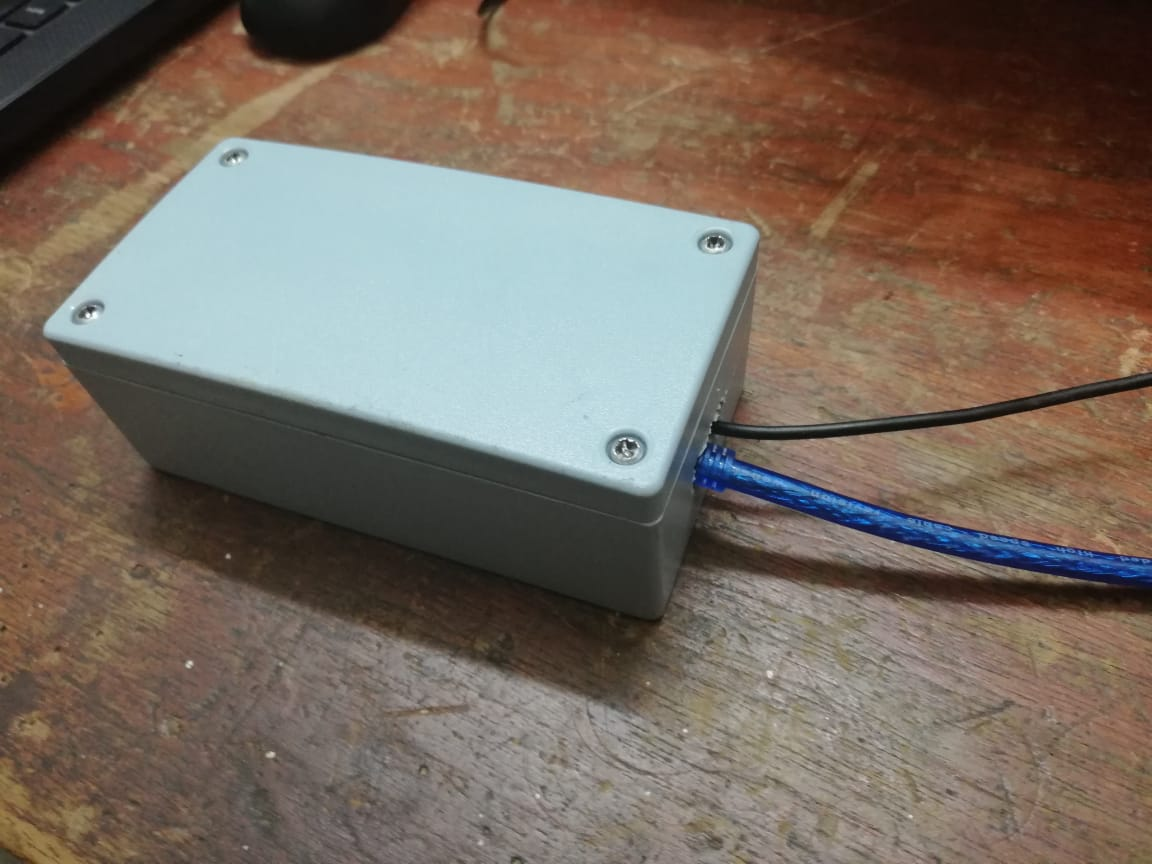
\includegraphics[width = 6 cm]{Imagenes/cajita}
   \caption{Caja contenedora del data logger}
\end{figure}

\item Se colocaron los data loggers de los equipos en una estación de madera para protegerlos del sol (Figura 4), se colocó el sensor de temperatura en las latas(Figura 5). Es importante mencionar que algunos equipos realizaron ademas la medición de temperatura ambiente con el sensor analógico LM35.

\begin{figure}[h]
   \centering
   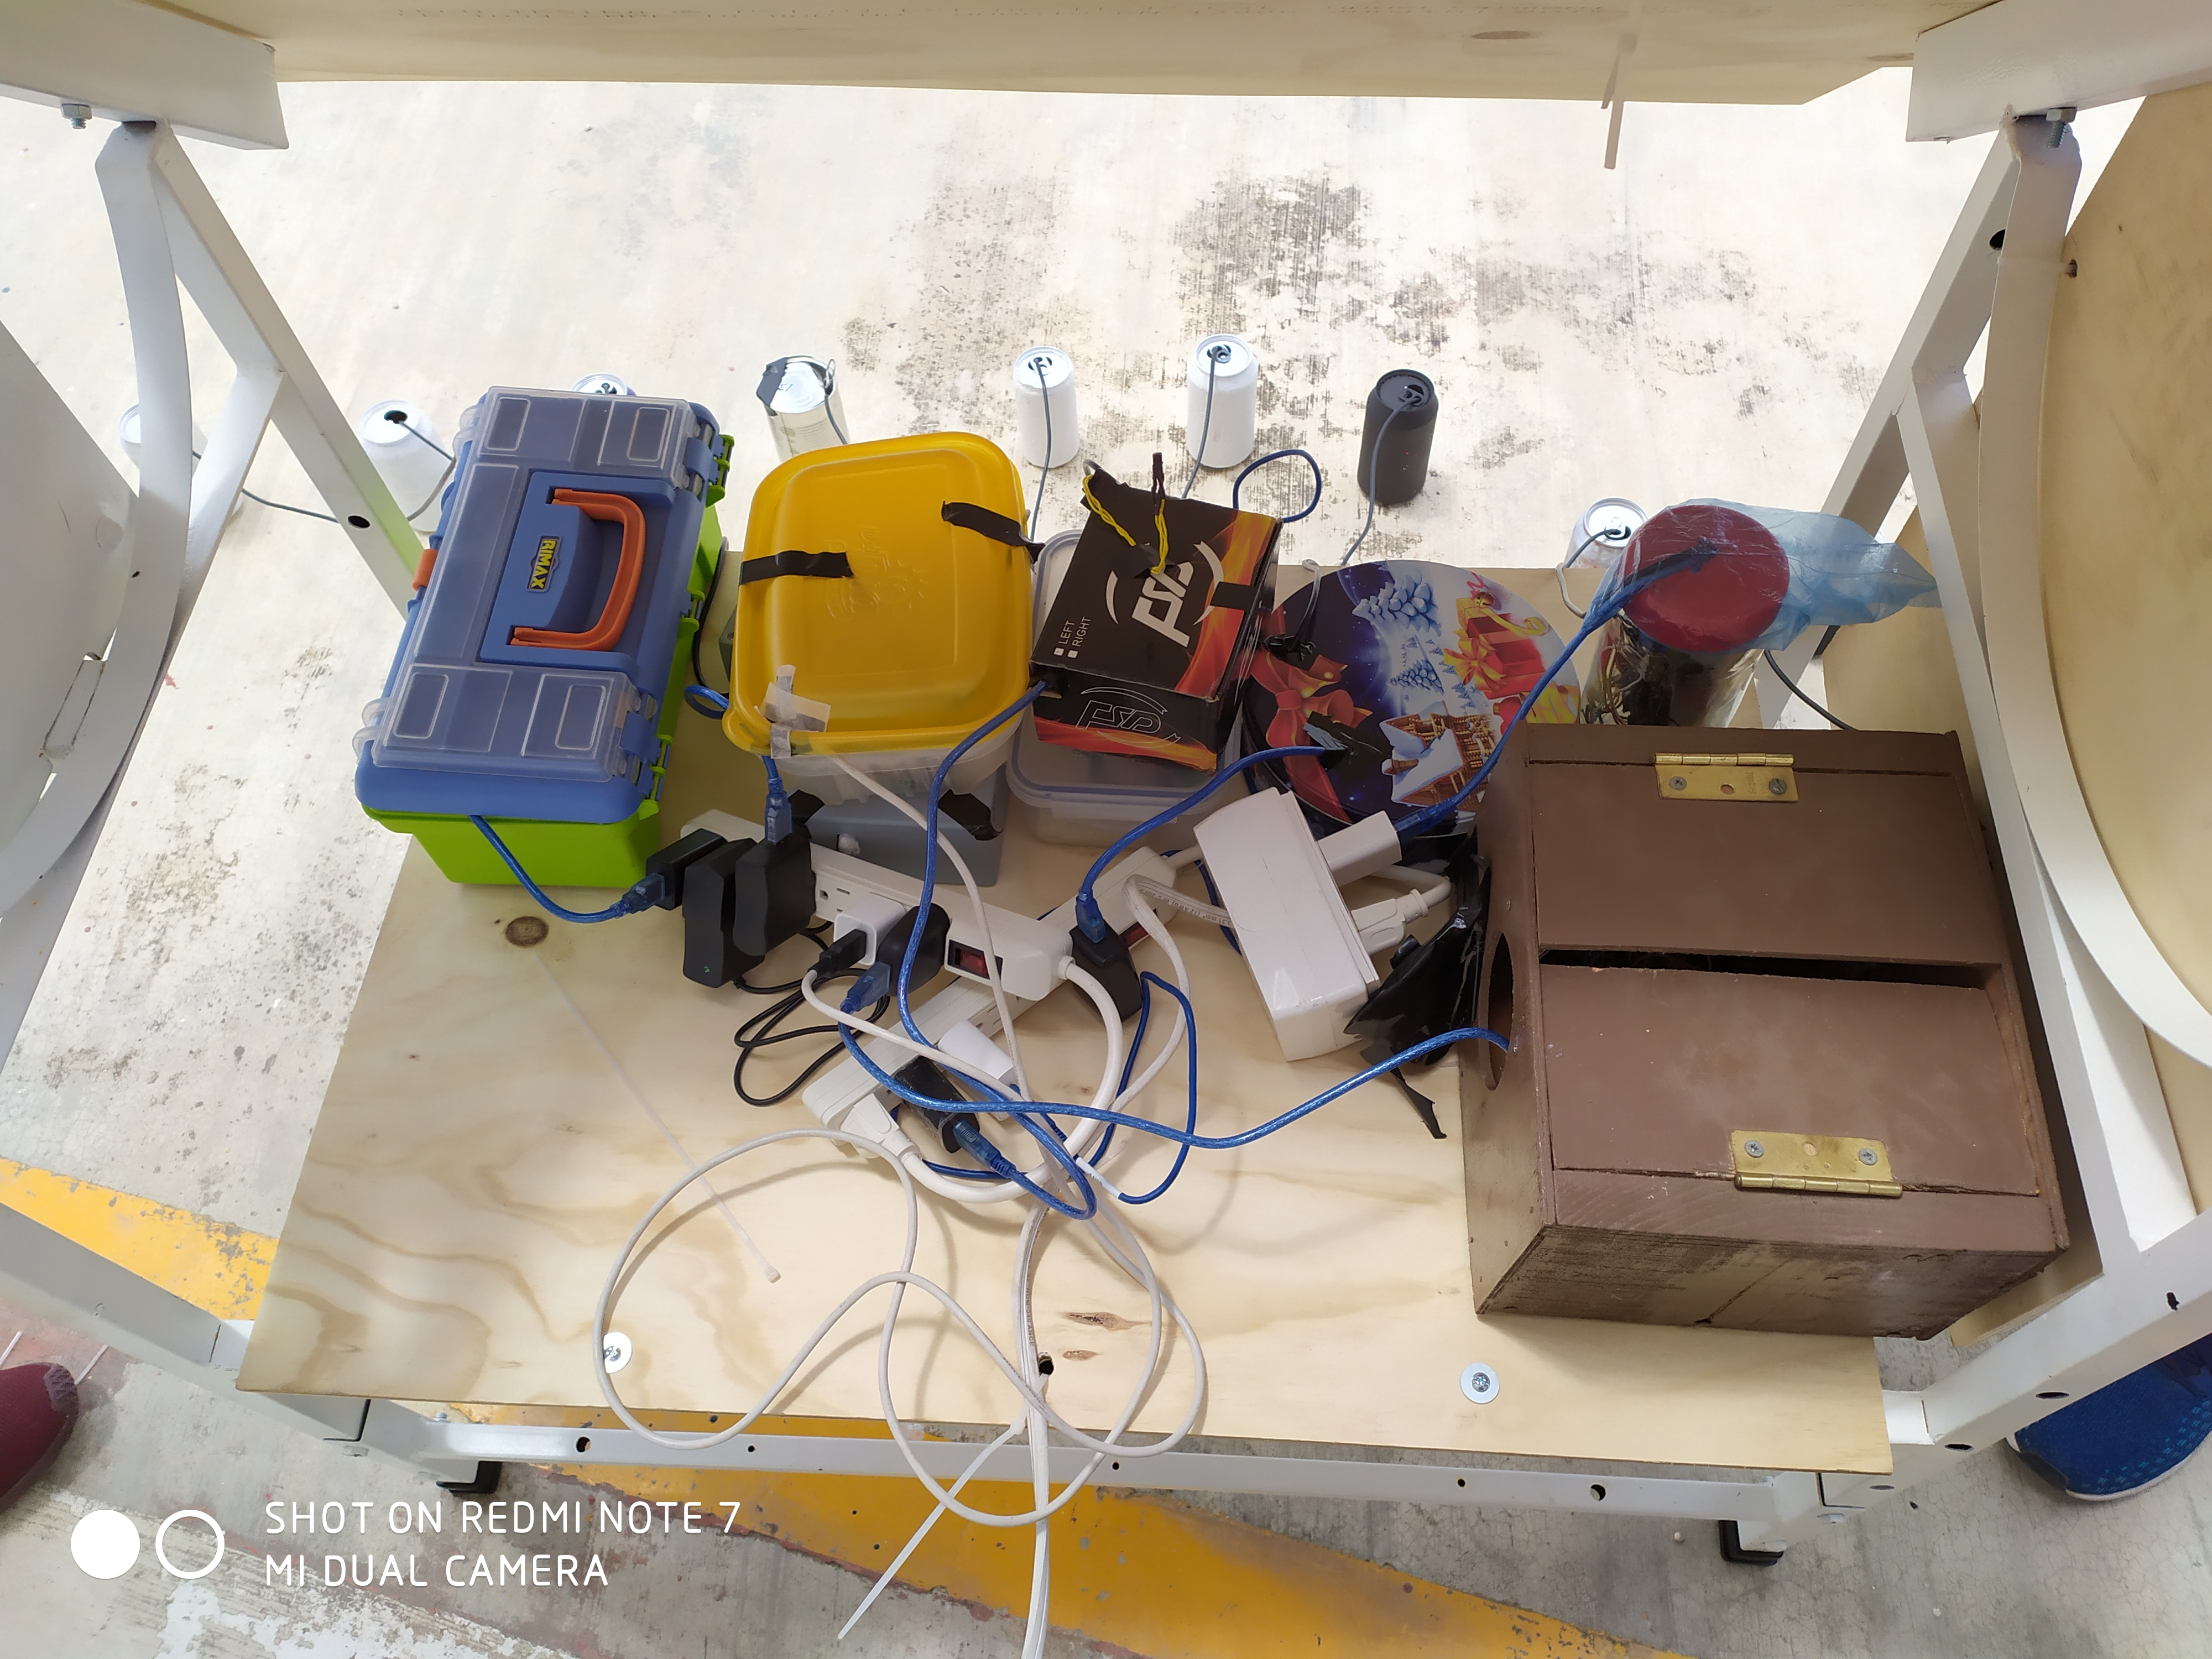
\includegraphics[width = 6 cm]{Imagenes/estacion}
   \caption{Estación de data loggers conectados a la corriente}
\end{figure}

\item Un día después de haberse colocado, a la hora de la clase, se retiraron los data loggers y se extrajeron los archivos de texto con los datos adquiridos. El profesor colocó los archivos de cada equipo en la carpeta de Google Drive utilizada para descargas los materiales de la asignatura.

\begin{figure}[h]
   \centering
   \includegraphics[width = 6 cm, height = 3.8 cm ]{Imagenes/latas}
   \caption{Latas de los equipos siendo sensadas por el DS18B20}
\end{figure}

\end{enumerate}

\section*{Resultados y discusión}

Utilizando el lenguaje de programación Python y las librerias, numpy, scipy y matplotlib, se realizó el análisis de datos de los datos de cada uno de los equipos a la vez. La Figura 6 muestra gráficas de las temperaturas medidas y de la temperatura ambiente si es que fue realizada.

\begin{figure*}[hbt!]
   \centering
   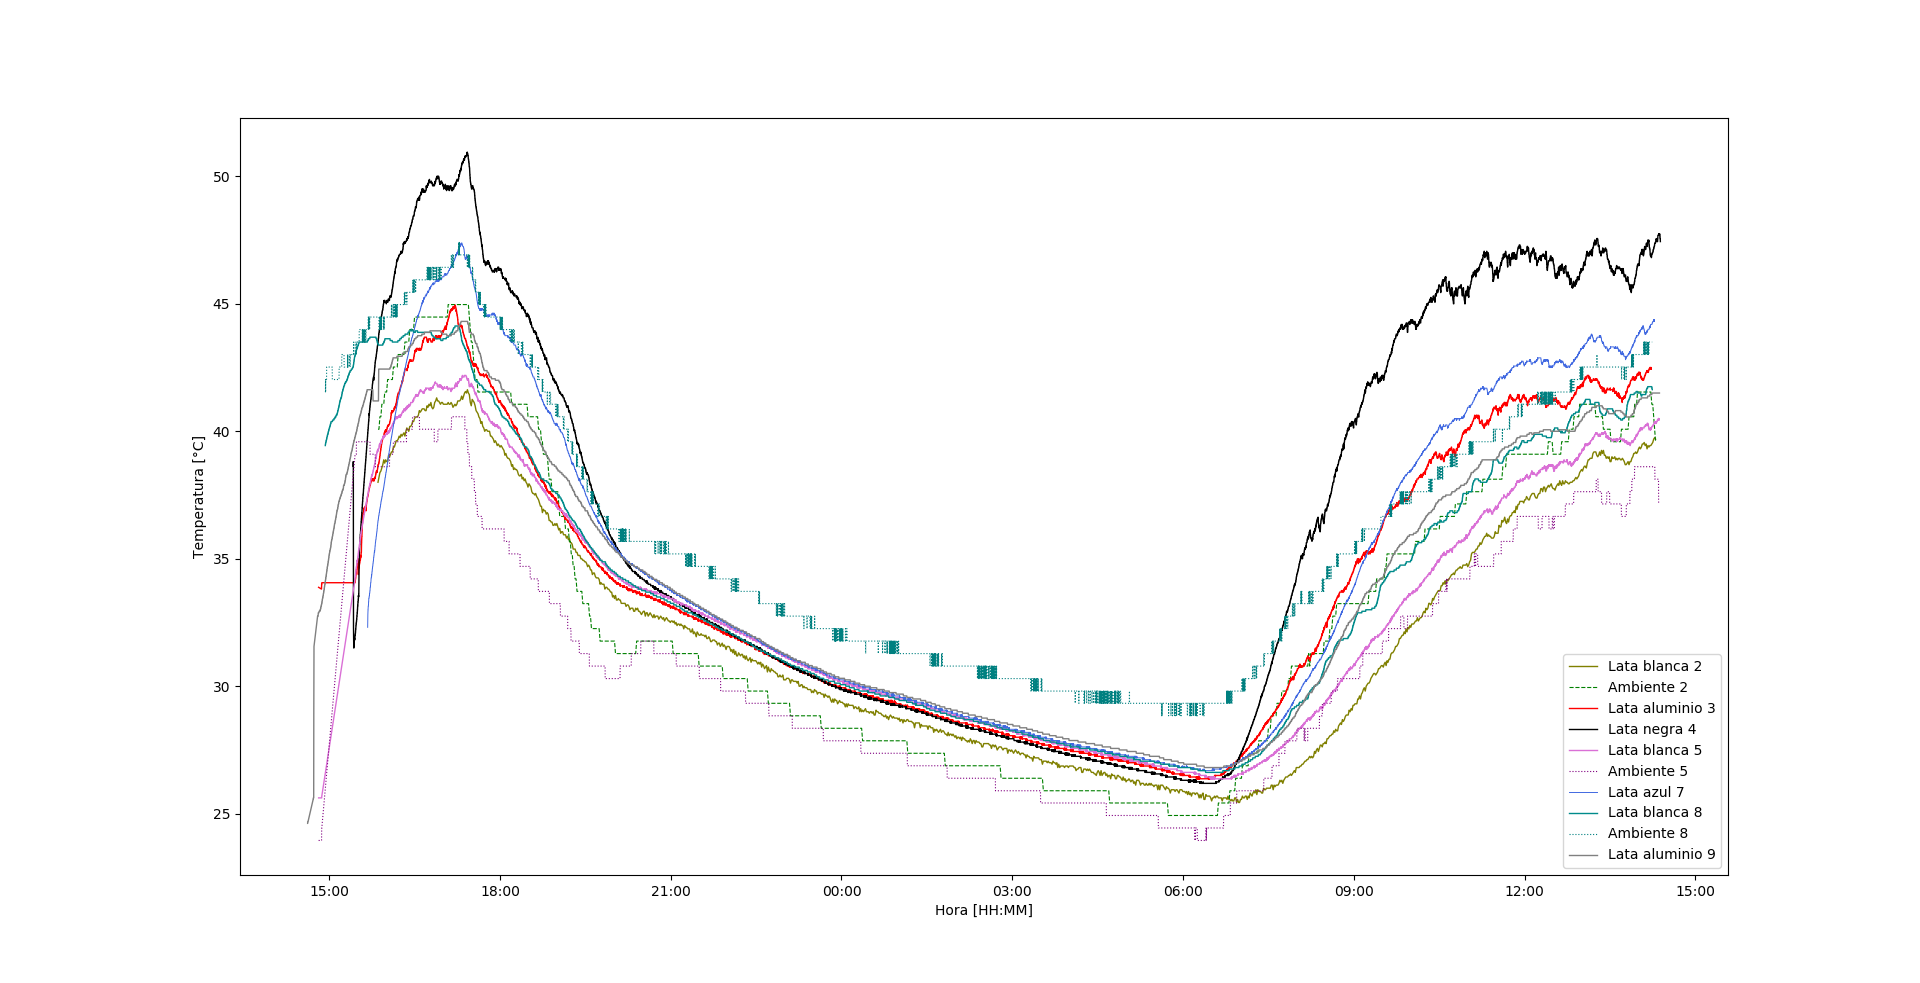
\includegraphics[width = 18 cm]{Imagenes/curvas}
   \caption{Comparación de curvas de temperatura}
\end{figure*}

Al observar la gráfica podemos notar que la lata pintada de negro fue la que mayor temperatura alcanzó, al mirar en la gráfica las que fueron pintadas de blanco, notamos una temperatura más baja , mientras que la lata azul y las de aluminio sin pintar se encuentran en el medio de estos dos extremos.

Al mirar el eje de abscisas, en donde se señala la hora y minuto del día a la que se midió una determinada temperatura, es observable que las mayores temperaturas se pudieron registrar a las horas en las que el sol irradiaba calor directamente sobre las latas, con lo que podemos decir que nuestras hipótesis fueron acertadas.


\section*{Conclusión}

Podemos ver que los data logger en general funcionaron correctamente y de acuerdo a lo esperado, guardando correctamente la fecha y hora junto con la información de los sensores. Podemos asegurar entonces que este se traducirá correctamente en futuros proyectos que requiera el registro de datos con esta configuración.

\bibliographystyle{apacite}

\bibliography{ref}

\end{document}
